\documentclass[a4paper,headsepline=3pt,headinclude=true,12pt,oneside]{scrartcl}
\usepackage[left=2cm,right=2cm,top=1cm,bottom=3cm,includeheadfoot]{geometry}
\usepackage{scrlayer-scrpage}
\usepackage{mwe}
\usepackage[origlayout=true,automark,colors={bvm}]{URpagestyles}
    \definecolor{UR@color@10}{HTML}{800000}
    \definecolor{redA}{HTML}{800000}
    \definecolor{grayA}{HTML}{9c9c9c}
    \definecolor{grayB}{HTML}{696969}
    \definecolor{grayC}{HTML}{404040}
    
\usepackage{lipsum} %fuer Fuelltexte

\usepackage{iftex}%automatische Auswahl des richtigen Fontloaders und der Eingabekodierung
%Es liefert das Makro \ifPDFTeX. Die Abfragen können entfernt werden, wenn nur eine bestimmte Variante verwendet wird.
\ifPDFTeX%falls mit pdfLaTeX kompiliert wird
	\usepackage[utf8]{inputenc}
	\usepackage[T1]{fontenc}
	\usepackage[ngerman]{babel} 
	%\usepackage[english]{babel} %Sparache aendern
\else%falls mit Lua oder XeLaTeX kompiliert wird
	\usepackage{fontspec}
	\usepackage{polyglossia}
	\setmainlanguage{english} 
\fi
\usepackage{lmodern} %moderne Schriftarten
\usepackage{csquotes}
\usepackage{titletoc} %partielles Inhaltsverzeichnis

%alles mit Tabellen
\usepackage{array}
\usepackage{booktabs}
\usepackage{longtable}
\usepackage{csvsimple}
\usepackage{multirow}
\usepackage{makecell}

\usepackage{xspace} %Abstaende
\usepackage{setspace} %Zeilenabstand

%alles mit Bildern
\usepackage{float}
\usepackage{placeins}
\usepackage{graphicx}
\usepackage{caption}
\usepackage{subcaption}
\usepackage{sidecap}
\usepackage{wrapfig}
\usepackage{pdfpages}

%alles mit Mathematik
\DeclareMathSizes{18}{18}{18}{18}
\usepackage{bbold}
\usepackage{dsfont}
\usepackage{upgreek}
\usepackage{paralist}
\usepackage{amsmath}
\usepackage{amssymb}
\usepackage{amscd}
\usepackage{siunitx}
\usepackage{thmtools}
\usepackage{pgfplots}
\pgfplotsset{compat=1.16}

%code texen
\usepackage{listings}
\lstset{ %Beispielkonfiguration fuer C-code
  backgroundcolor=\color{lightgray!50!white},   % choose the background color; you must add \usepackage{color} or \usepackage{xcolor}; should come as last argument
  basicstyle=\footnotesize,        % the size of the fonts that are used for the code
  breakatwhitespace=false,         % sets if automatic breaks should only happen at whitespace
  breaklines=true,                 % sets automatic line breaking
  captionpos=b,                    % sets the caption-position to bottom
  commentstyle=\color{orange},     % comment style
  deletekeywords={sizeof},         % if you want to delete keywords from the given language
  extendedchars=true,              % lets you use non-ASCII characters; for 8-bits encodings only, does not work with UTF-8
  firstnumber=1,                   % start line enumeration with line 1000
  frame=single,                    % adds a frame around the code
  keepspaces=true,                 % keeps spaces in text, useful for keeping indentation of code (possibly needs columns=flexible)
  %keywordstyle=\color{red!50!black},% keyword style
  keywordstyle=\color{blue},% keyword style
  language=C++,                    % the language of the code
  morekeywords={__constant__, __shared__, __device__, __host__, __global__, __managed__, float2, float3, float4, dim3, int2, int3, int4, uint, half, cudaStream_t, cudaEvent_t, cudaError_t, cudnnError_t, cusparseError_t, cublasError_t, curandError_t, cufftError_t, cusolverError_t, __kernel, kernel, __constant, constant, __local, local, __private, private, __global, global, cl_device_id, cl_platform_id, cl_int, cl_uint, cl_float, cl_double, string, cl_mem, cl_kernel, size_t, cl_event, cl_program, cl_context, cl_command_queue, FILE, restrict, event_t, ptrdiff_t , intptr_t, uintptr_t, device_ptr, device_vector, host_vector, vector, Platform, Context, CommandQueue, Buffer, Program, Kernel, Sources, Device, cl_context_properties, hipStream_t, cufftHandle, cufftComplex, cufftReal, cufftDouble, cufftDoubleComplex, clfftSetupData, clfftDim, fftw_complex, fftw_plan, curandStateSobol32_t, curandStateScrambledSobol32_t, curandStateSobol64_t, curandStateScrambledSobol64_t, curandState (XORWOW), curandStatePhilox4_32_10_t, curandStateMRG32k3a, curandStateMtgp32_t, curandGenerator_t, curandState, clrngMrg31k3pHostStream, clrngMrg31k3pStream, clprobdistExponential, clqmcLatticeRule, clqmcLatticeRuleStream, cublasHandle_t, cublasOperation_t, cuComplex, cuDoubleComplex, clsparseIdx_t, cldenseVector, clsparseCreateResult, clsparseCreateSolverResult, clsparseCsrMatrix, cusolverDnHandle_t, cusolverSpHandle_t, cusolverRfHandle_t, magma_queue_t, magma_int_t, LocalVector, CG, LocalStencil, __attribute__, aligned_allocator, auto, tensorflow, trt, tf, keras, Mat, cudnnHandle_t, cudnnTensorDescriptor_t, cudnnFilterDescriptor_t, cudnnConvolutionDescriptor_t, cudnnConvolutionFwdAlgo_t, ncclComm_t, MPI_INT},% if you want to add more keywords to the set
  numbers=left,                    % where to put the line-numbers; possible values are (none, left, right)
  numbersep=5pt,                   % how far the line-numbers are from the code
  numberstyle=\small\color{black}, % the style that is used for the line-numbers
  rulecolor=\color{black},         % if not set, the frame-color may be changed on line-breaks within not-black text (e.g. comments (green here))
  showspaces=false,                % show spaces everywhere adding particular underscores; it overrides 'showstringspaces'
  showstringspaces=false,          % underline spaces within strings only
  showtabs=false,                  % show tabs within strings adding particular underscores
  stepnumber=2,                    % the step between two line-numbers. If it's 1, each line will be numbered
  stringstyle=\color{green!50!black}, % string literal style
  identifierstyle=\color{black},
  tabsize=2,	                   % sets default tabsize to 2 spaces
  title=\lstname                   % show the filename of files included with \lstinputlisting; also try caption instead of title
}
\expandafter\ifx\csname li\endcsname\relax
\let\li=\lstinline
\else\errmessage{li schon definiert \meaning\li}%
\fi

%Literaturverzeichnis
\usepackage[backend=biber, citestyle=numeric, bibstyle=numeric]{biblatex}
\addbibresource{lit/lit.bib} %richtigen Pfad ersetzen

\setlength{\parindent}{0pt} %keine Absatzeinzüge
\setlength{\parskip}{\baselineskip}

%Links
\usepackage[colorlinks=true,
            linkcolor=black,
            urlcolor=gray,
            citecolor=gray,
            bookmarks=true]{hyperref}
\usepackage{tabularx} %Tabellencounter, nach hyperref

\DeclareCaptionFont{black}{\color{black}}
\DeclareCaptionFormat{listing}{
  \colorbox[rgb]{1,1,1}{
    \parbox{\textwidth}{\hspace{15pt}#1#2#3}
  }
}
\captionsetup[lstlisting]{format=listing, labelfont=black, textfont=black, singlelinecheck=false, margin=0pt, font={bf,footnotesize}}

\renewcommand*{\familydefault}{\sfdefault}
\newcommand*{\pck}[1]{\texttt{#1}}
\newcommand*{\code}[1]{\texttt{#1}}
\newcommand*{\repl}[1]{\textrm{\textit{#1}}}
\newcommand{\cmd}[1]{\par\medskip\noindent\fbox{\ttfamily#1}\par\medskip\noindent}
\setcounter{secnumdepth}{\sectionnumdepth}
\newsavebox{\remarkbox}
\sbox{\remarkbox}{\emph{Remark:~}}
\newcounter{iterator}
\usepackage{colortbl}

%meta Informationen
\author{Thomas Karl}
\title{Computation of Zero Points with Weierstraß Iteration in OpenCL 3.0}
\subtitle{University of Regensburg}
\date{\today}
%\renewcommand{\titlepagestyle}{URtitle} 

\cfoot*{ }
\ofoot*{\thepage}% the pagenumber in the center of the foot, also on plain pages
\ihead*{ }% Name and title beneath each other in the inner part of the foot
\ohead*{\headmark}
\automark[subsection]{section}

\newcommand*\Laplace{\mathop{}\!\mathbin\bigtriangleup}

\begin{document}
\begin{onehalfspace}

	\maketitle
	\thispagestyle{empty}
		
	\section{Setup}
	The program computes complex zero points of arbitrary complex polynomials numerically using Weierstraß Iteration. The procedure is accelerated on GPUs with OpenCL 1.2. Inputs are the number of polynomials $n$ and its degree $d$. Let $p$ be the number of cores. The number of polynomials $n_p$ that can be computed in parallel is $n_p=\lfloor p/d \rfloor$. If $dn_p \neq p$, some cores remain idle.
	
	Each core computes an initial guess and randomly a complex coefficient for the polynomial. Real- and imaginary part lie uniformly distributed between two parameters that where also given as user input. The zero points have to be complex and lie in the initially on a circle in the complex plane. The radius is the half distance between the parameters.
	
	Each core improves its $k$-th zero point $x_k$ using the iteration, 
	
	\begin{equation}
		x_k^{i+1} = x_k + \frac{\text{polynomial}(x_k^i)}{\prod_{j=1;j\neq k}^{d}(x_k^i-\zeta_j)} \longrightarrow x_k \qquad i \rightarrow \infty
	\end{equation}

	$\zeta_j$ denote all zero points so far. Since a dynamically change of the $\zeta_j$ in each iteration accelerates the convergence, dataraces can be ignored,
	
	The iteration breaks after $10d$ runs or if for a a user given $\varepsilon > 0$ the equation	
	
	\begin{equation}
		\text{max}\left\{ \frac{|\text{polynomial}(x)|}{|x|} \right\} \leq \varepsilon
	\end{equation}
	
	holds. This iteration is commonly known as \textit{Weierstraß-Durand-Kerner} Iteration. The zero points are converted in coordinates in a $1080\times 1080$ pixel image and generated on the CPU in \textit{ppm} format. Figure \ref{img} shows an example.

	
	\section{Evaluation}
	For the evaluation of the performance the computation times where recorded and fitted linearly. Figure \ref{plot1} shows the comparison of computation times on a CPU and a GPU. The GPU was a \textit{Nvidia GTX 1060}, the CPU an \textit{Intel i7 8700K 4.8GHz}. Using 1280 cores we get a speedup with respect to the serial program of roughly $70$. The latency due to the data traffic reads about $0.5$ seconds.
	
	\begin{figure}[h]
		\centering
		  \begin{tikzpicture}[scale=1.15]
  \scriptsize
    \begin{loglogaxis}[xlabel={number of polynomials $n$}, ylabel={computation time $t$ / sec.}, legend pos=outer north east, legend style={cells={align=left}}]
      \addplot [draw=red!50!black, mark=*, only marks, fill=red!50!white] table[x expr=\thisrowno{0},y index=3]{test/time.dat};
      \addlegendentry{GPU}
      \addplot [draw=lightgray!50!black, mark=*, only marks, fill=lightgray!50!white] table[x expr=\thisrowno{0},y index=7]{test/time.dat};
      \addlegendentry{CPU}    
      \addplot [domain=8000:150000, color=red!50!black, line width=1pt, mark=none] {3.29792237e-06*x+1.46283417e-01};
      \addlegendentry{$t(n) = \SI{3.298e-6}\cdot n+0.146$};         
      \addplot [domain=8000:150000, color=lightgray!50!black, line width=1pt, mark=none] {0.00024319*x+0.01357063};
      \addlegendentry{$t(n) = \SI{243.2e-6}\cdot n+0.014$};
          
    \end{loglogaxis}
  \end{tikzpicture}
%[0.00024319 0.01357063]
%[3.29792237e-06 1.46283417e-01]
		%\includegraphics[width=\textwidth]{doc/wdk1.png}
		\caption{Computation times for certain numbers of polynomials.}
		\label{plot1}
	\end{figure}
	
	\newpage
	
	In the last step the dependency of the polynomial degree is evaluated (Fig. \ref{plot2}). When the degree is doubled, for the same number of polynomials twice the number of zero points needs to be computed. The number of floating point operations and the iterations increase also with the degree. When the computation times are compared for the same number of zero points ($n\cdot d$) For degree 8 to 32 the computation time is almost the same for a larger number of polynomials.
	
	\begin{figure}[h]
		\centering
		  \begin{tikzpicture}[scale=1.15]
  \scriptsize
    \begin{loglogaxis}[xlabel={number of zero points $d\cdot n$}, ylabel={computation time $t$ / sec.}, legend pos=outer north east, legend style={cells={align=left}}]
      %\addplot [draw=red!50!black, mark=*, only marks, fill=red!50!white] table[x expr=\thisrowno{0}*8,y index=1]{test/time.dat};
      %\addlegendentry{degree 8}
      %\addplot [draw=gray!50!black, mark=*, only marks, fill=gray!50!white] table[x expr=\thisrowno{0}*16,y index=2]{test/time.dat};
      %\addlegendentry{degree 16} 
      \addplot [draw=lightgray!50!black, mark=*, only marks, fill=lightgray!50!white] table[x expr=\thisrowno{0}*32,y index=3]{test/time.dat};
      \addlegendentry{degree 32}  
      \addplot [draw=red!50!black, mark=*, only marks, fill=red!80!white] table[x expr=\thisrowno{0}*64,y index=4]{test/time.dat};
      \addlegendentry{degree 64}
      %\addplot [draw=red!50!black, mark=*, only marks, fill=red!50!white] table[x expr=\thisrowno{0}*128,y index=5]{test/time.dat};
      %\addlegendentry{degree 128}
      \addplot [draw=gray!50!black, mark=*, only marks, fill=gray!50!white] table[x expr=\thisrowno{0}*256,y index=6]{test/time.dat};
      \addlegendentry{degree 256} 
      %\addplot [domain=60000:100000000, color=red!50!black, line width=1pt, mark=none] {1.17156954e-07*x+1.10557375e-01};
      %\addlegendentry{$t(n) = \SI{1.17e-7}\cdot dn+0.11$};
      %\addplot [domain=60000:100000000, color=gray!50!black, line width=1pt, mark=none] {1.11224937e-07*x+1.23205917e-01};
      %\addlegendentry{$t(n) = \SI{1.11e-7}\cdot dn+0.12$};
      \addplot [domain=60000:100000000, color=lightgray!70!black, line width=1pt, mark=none] {1.03060074e-07*x+1.46283417e-01};
      \addlegendentry{$t(n) = \SI{10.3e-6}\cdot dn+0.15$};      
      \addplot [domain=60000:100000000, color=red!80!white, line width=1pt, mark=none] {1.63081332e-06*x+5.74288542e-01};
      \addlegendentry{$t(n) = \SI{1.63e-6}\cdot dn+0.57$};
      %\addplot [domain=60000:100000000, color=red!50!black, line width=1pt, mark=none] {1.83507442e-06*x+1.60958004e+00};
      %\addlegendentry{$t(n) = \SI{1.84e-6}\cdot dn+1.61$}; 
      \addplot [domain=60000:100000000, color=gray!50!black, line width=1pt, mark=none] {2.23608397e-06*x+2.75923604e+00};
      \addlegendentry{$t(n) = \SI{2.23e-6}\cdot dn+2.76$}; 
    \end{loglogaxis}
  \end{tikzpicture}
		%\includegraphics[width=\textwidth]{doc/wdk2.png}
		\caption{Computation times for certain number of polynomials.}
		\label{plot2}
	\end{figure}
	
	\begin{figure}[h]
		\begin{subfigure}{0.5\textwidth}
		    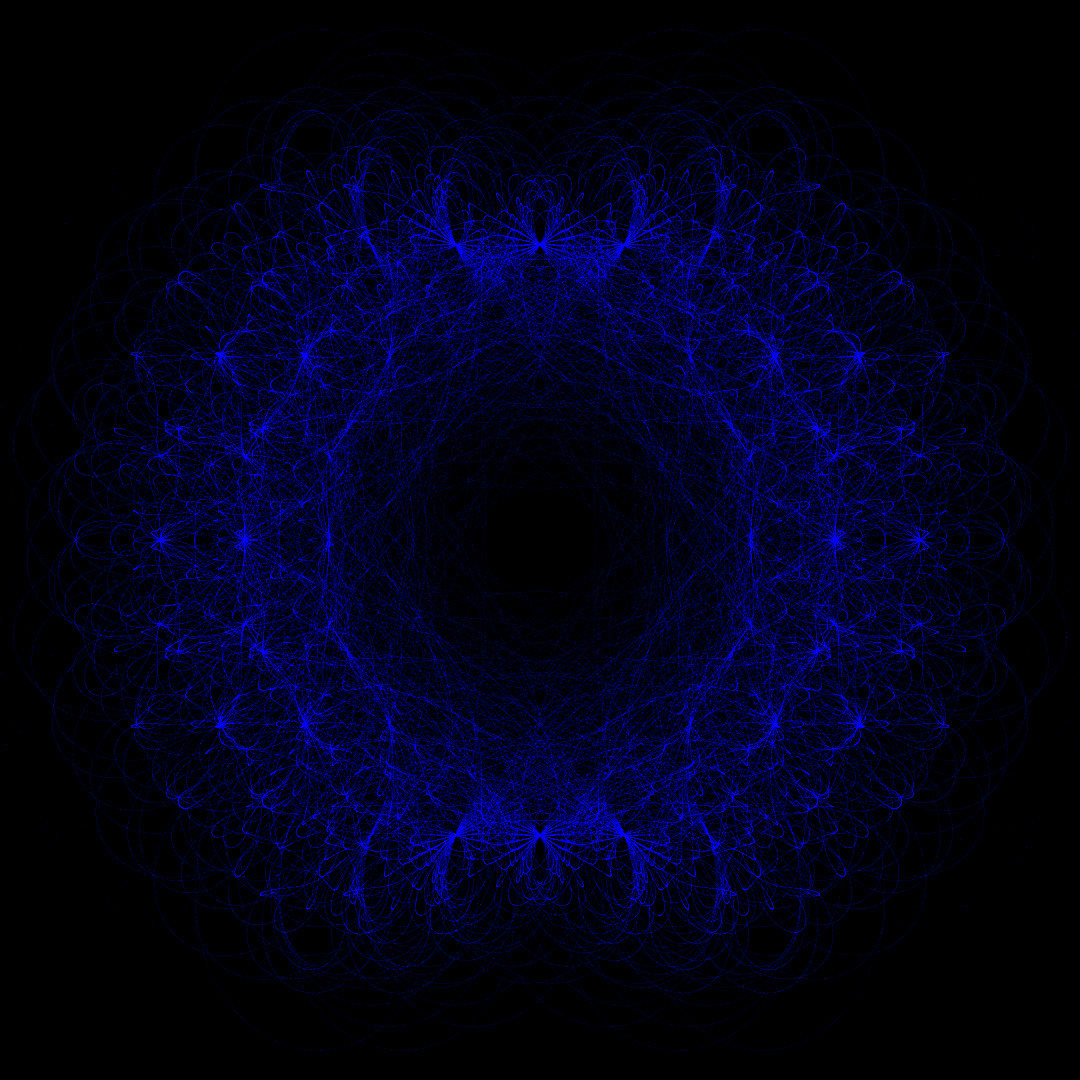
\includegraphics[width=\textwidth]{doc/deg8Impm30M.jpg}
		    \subcaption*{$n=\SI{30e6}{}$, $d=8$, imaginary part 1 or -1}
		\end{subfigure}\hfill
        \begin{subfigure}{0.5\textwidth}
		    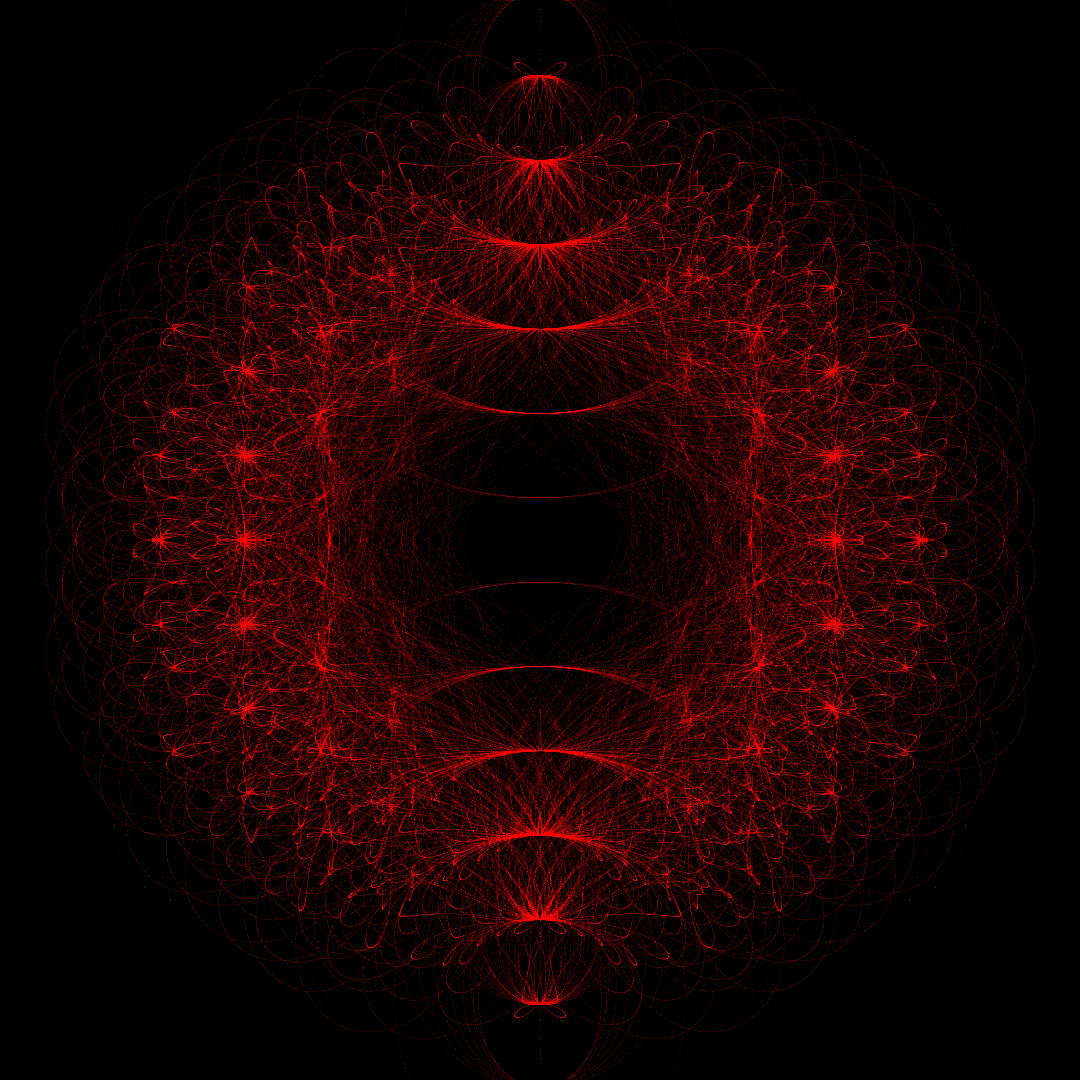
\includegraphics[width=\textwidth]{doc/deg8Repm30M.jpg}
		    \subcaption*{$n=\SI{30e6}{}$, $d=8$, real part 1 or -1}
		\end{subfigure}

		\begin{subfigure}{0.5\textwidth}
		    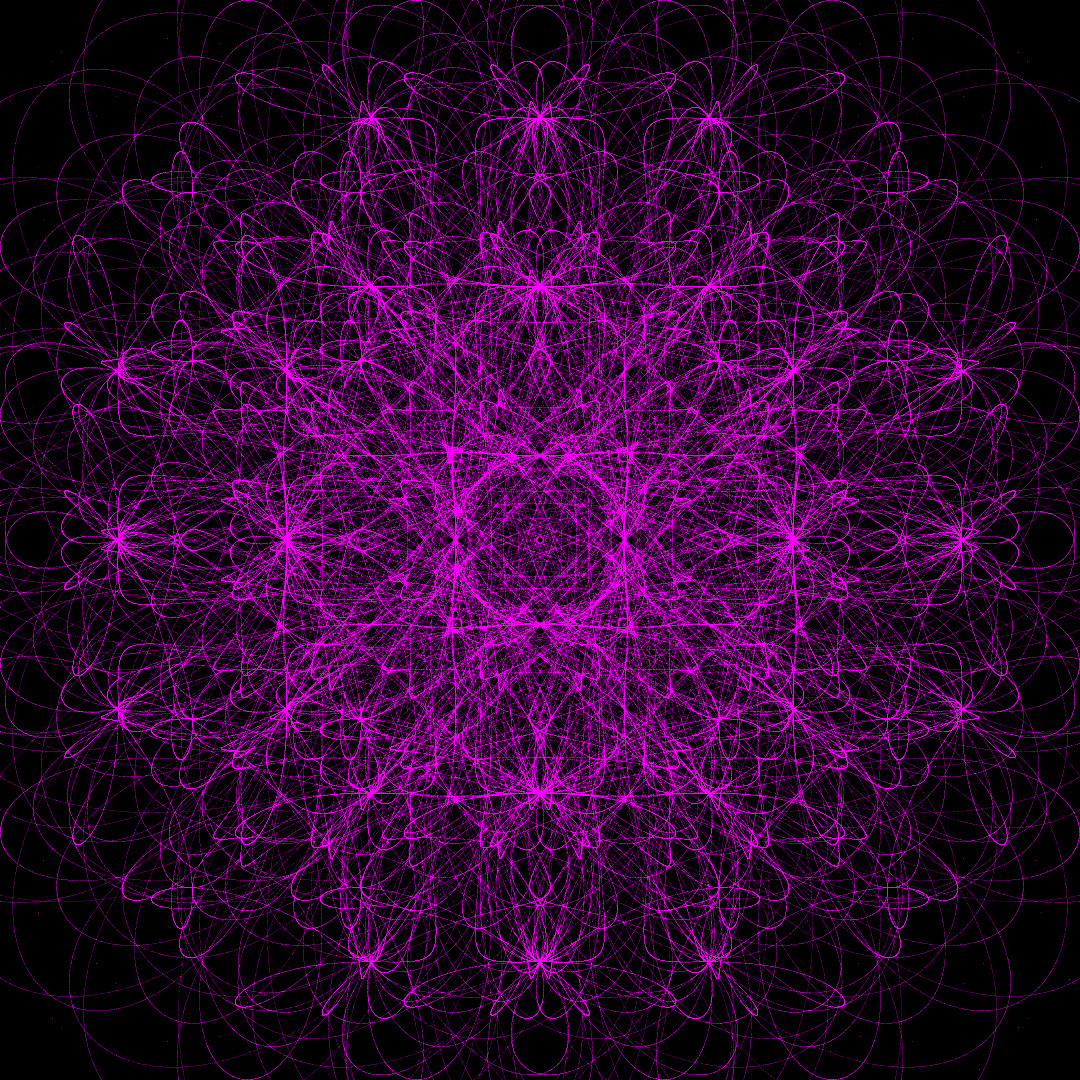
\includegraphics[width=\textwidth]{doc/deg4Both60M.jpg}
		    \subcaption*{$n=\SI{60e6}{}$, $d=4$, real and imaginary part 1 or -1, }
		\end{subfigure}\hfill
		\begin{subfigure}{0.5\textwidth}
		    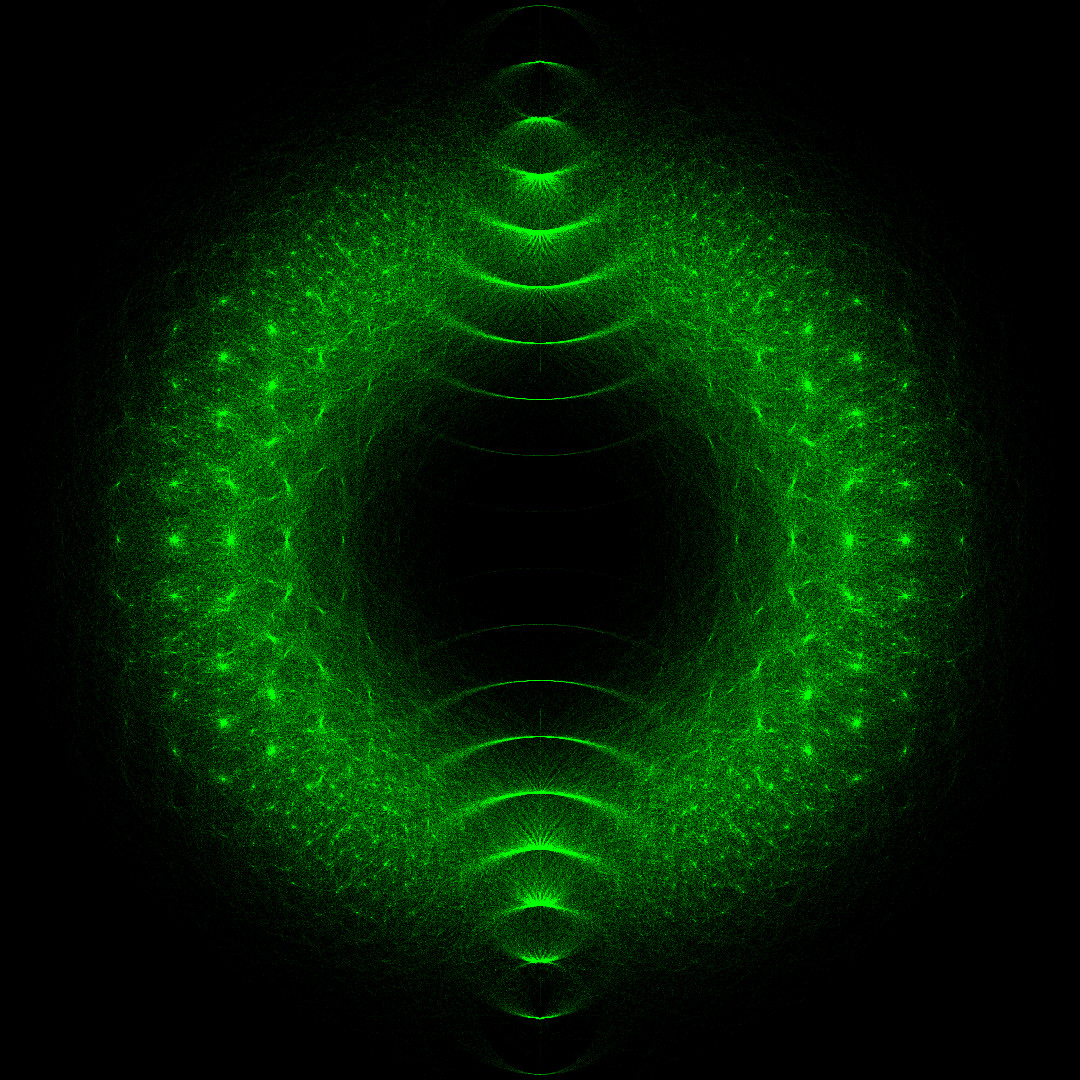
\includegraphics[width=\textwidth]{doc/deg12Repm40M.jpg}
		    \subcaption*{$n=\SI{40e6}{}$, $d=12$, real part 1 or -1}
		\end{subfigure}
		\caption{Graphical representation of zero points in complex plane ($1080\times 1080$ pixel, $\varepsilon=0.0001$). The zero points are distributed on a circle with radius one.}
		\label{img}
	\end{figure}
	
\end{onehalfspace}
\end{document}